\documentclass[12pt, a4paper]{article}
\title{Chapter 1}
\author{Maciej Harbuz}
\usepackage{amssymb}
\usepackage{amsmath}
\usepackage{tikz} 
\usepackage{import}
\usepackage{float}
\newcommand{\Mod}[1]{\ (\mathrm{mod}\ #1)}
\usetikzlibrary{automata, positioning, arrows}
\includeonly{chapter01-problems-150-159.tex}
\tikzset{
    ->, % makes the edges directed
    every state/.style={thick, fill=gray!15}, % sets the properties for each ’state’ node
    node distance=2.5cm, % specifies the minimum distance between two nodes. Change if necessary.
    initial text=$ $, % sets the text that appears on the start arrow
    >=stealth, % makes the arrow heads bold
}

\begin{document}

\maketitle

\section{Exercises}
\begin{enumerate}

    \item [1.19]
          Use the procedure described in Lemma 1.55 to convert the following regular expressions to nondeterministic finite automata.
          \begin{enumerate}
              \item $(0 \cup 1)^\ast000(0 \cup 1)^\ast$
                    \begin{figure}[H]
                        \centering
                        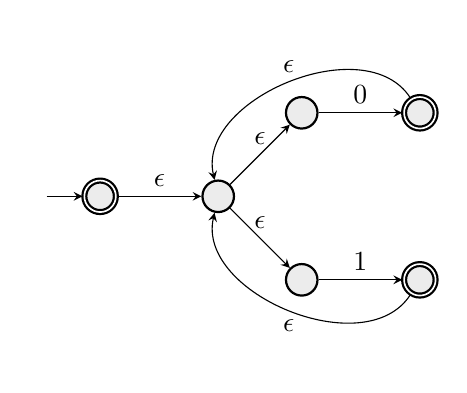
\begin{tikzpicture}[
                                styleSmall/.style={minimum size=4mm},
                                node distance=1.5cm,
                            ]
                            \node[state, accepting, initial, styleSmall] (q01asts) {};
                            \node[state, styleSmall, right of=q01asts] (q01sum) {};
                            \node[state, above right of=q01sum, styleSmall] (q01sum0) {};
                            \node[state, accepting, right of=q01sum0, styleSmall] (q01sum00) {};
                            \node[state, below right of=q01sum, styleSmall] (q01sum1) {};
                            \node[state, accepting, right of=q01sum1, styleSmall] (q01sum11) {};
                            \draw
                            (q01asts) edge[above] node{$\epsilon$} (q01sum)
                            (q01sum) edge[above] node{$\epsilon$} (q01sum0)
                            (q01sum) edge[above] node{$\epsilon$} (q01sum1)
                            (q01sum0) edge[above] node{$0$} (q01sum00)
                            (q01sum1) edge[above] node{$1$} (q01sum11)
                            (q01sum00) edge[bend right=80, above] node{$\epsilon$} (q01sum)
                            (q01sum11) edge[bend left=80, below] node{$\epsilon$} (q01sum);
                        \end{tikzpicture}
                        \caption{$(0 \cup 1)^\ast$}
                    \end{figure}
                    \begin{figure}[H]
                        \centering
                        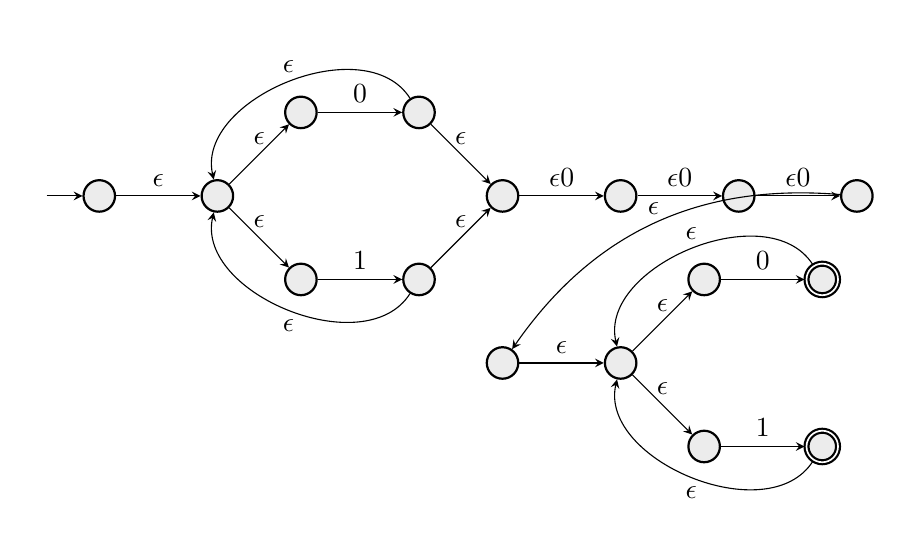
\begin{tikzpicture}[
                                styleSmall/.style={minimum size=4mm},
                                node distance=1.5cm,
                            ]
                            \node[state, initial, styleSmall] (q01asts) {};
                            \node[state, styleSmall, right of=q01asts] (q01sum) {};
                            \node[state, above right of=q01sum, styleSmall] (q01sum0) {};
                            \node[state, right of=q01sum0, styleSmall] (q01sum00) {};
                            \node[state, below right of=q01sum, styleSmall] (q01sum1) {};
                            \node[state, right of=q01sum1, styleSmall] (q01sum11) {};

                            \node[state, below right of=q01sum00, styleSmall] (qzs) {};
                            \node[state, right of=qzs, styleSmall] (qz0) {};
                            \node[state, right of=qz0, styleSmall] (qz00) {};
                            \node[state, right of=qz00, styleSmall] (qz000) {};

                            \node[state, below right of=q01sum11, styleSmall] (q21asts) {};
                            \node[state, styleSmall, right of=q21asts] (q21sum) {};
                            \node[state, above right of=q21sum, styleSmall] (q21sum0) {};
                            \node[state, accepting, right of=q21sum0, styleSmall] (q21sum00) {};
                            \node[state, below right of=q21sum, styleSmall] (q21sum1) {};
                            \node[state, accepting, right of=q21sum1, styleSmall] (q21sum11) {};
                            \draw
                            (q01asts) edge[above] node{$\epsilon$} (q01sum)
                            (q01sum) edge[above] node{$\epsilon$} (q01sum0)
                            (q01sum) edge[above] node{$\epsilon$} (q01sum1)
                            (q01sum0) edge[above] node{$0$} (q01sum00)
                            (q01sum1) edge[above] node{$1$} (q01sum11)
                            (q01sum00) edge[bend right=80, above] node{$\epsilon$} (q01sum)
                            (q01sum11) edge[bend left=80, below] node{$\epsilon$} (q01sum)

                            (q01sum00) edge[above] node{$\epsilon$} (qzs)
                            (q01sum11) edge[above] node{$\epsilon$} (qzs)

                            (qzs) edge[above] node{$\epsilon0$} (qz0)
                            (qz0) edge[above] node{$\epsilon0$} (qz00)
                            (qz00) edge[above] node{$\epsilon0$} (qz000)

                            (qz000) edge[above, bend right] node{$\epsilon$} (q21asts)

                            (q21asts) edge[above] node{$\epsilon$} (q21sum)
                            (q21sum) edge[above] node{$\epsilon$} (q21sum0)
                            (q21sum) edge[above] node{$\epsilon$} (q21sum1)
                            (q21sum0) edge[above] node{$0$} (q21sum00)
                            (q21sum1) edge[above] node{$1$} (q21sum11)
                            (q21sum00) edge[bend right=80, above] node{$\epsilon$} (q21sum)
                            (q21sum11) edge[bend left=80, below] node{$\epsilon$} (q21sum);
                        \end{tikzpicture}
                        \caption{$(0 \cup 1)^\ast000(0 \cup 1)^\ast$}
                    \end{figure}
              \item $(((00)^\ast(11)) \cup 01)^\ast$
                    \begin{figure}[H]
                        \centering
                        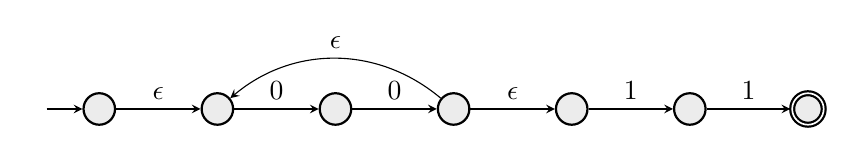
\begin{tikzpicture}[
                                styleSmall/.style={minimum size=4mm},
                                node distance=1.5cm,
                            ]
                            \node[state, initial, styleSmall] (q0e) {};
                            \node[state, styleSmall, right of=q0e] (q0) {};
                            \node[state, right of=q0, styleSmall] (q01) {};
                            \node[state, right of=q01, styleSmall] (q02) {};
                            \node[state, right of=q02, styleSmall] (q1e) {};
                            \node[state, right of=q1e, styleSmall] (q11) {};
                            \node[state, accepting, right of=q11, styleSmall] (q12) {};
                            \draw
                            (q0e) edge[above] node{$\epsilon$} (q0)
                            (q0) edge[above] node{$0$} (q01)
                            (q01) edge[above] node{$0$} (q02)
                            (q02) edge[bend right=40, above] node{$\epsilon$} (q0)
                            (q02) edge[above] node{$\epsilon$} (q1e)
                            (q1e) edge[above] node{$1$} (q11)
                            (q11) edge[above] node{$1$} (q12);
                        \end{tikzpicture}
                        \caption{$((00)^\ast(11))$}
                    \end{figure}
                    \begin{figure}[H]
                        \centering
                        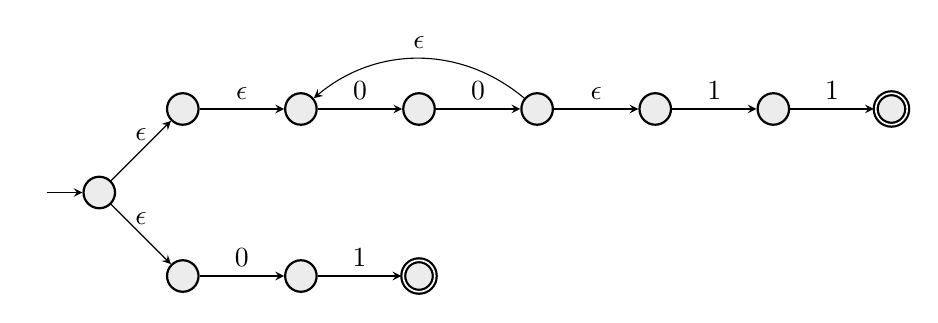
\begin{tikzpicture}[
                                styleSmall/.style={minimum size=4mm},
                                node distance=1.5cm,
                            ]
                            \node[state, initial, styleSmall] (qse) {};
                            \node[state, above right of=qse, styleSmall] (q0e) {};
                            \node[state, styleSmall, right of=q0e] (q0) {};
                            \node[state, right of=q0, styleSmall] (q01) {};
                            \node[state, right of=q01, styleSmall] (q02) {};
                            \node[state, right of=q02, styleSmall] (q1e) {};
                            \node[state, right of=q1e, styleSmall] (q11) {};
                            \node[state, accepting, right of=q11, styleSmall] (q12) {};
                            \node[state, below right of=qse, styleSmall] (qs1) {};
                            \node[state, right of=qs1, styleSmall] (qs2) {};
                            \node[state, accepting, right of=qs2, styleSmall] (qs3) {};
                            \draw
                            (q0e) edge[above] node{$\epsilon$} (q0)
                            (q0) edge[above] node{$0$} (q01)
                            (q01) edge[above] node{$0$} (q02)
                            (q02) edge[bend right=40, above] node{$\epsilon$} (q0)
                            (q02) edge[above] node{$\epsilon$} (q1e)
                            (q1e) edge[above] node{$1$} (q11)
                            (q11) edge[above] node{$1$} (q12)
                            (qse) edge[above] node{$\epsilon$} (q0e)
                            (qse) edge[above] node{$\epsilon$} (qs1)
                            (qs1) edge[above] node{$0$} (qs2)
                            (qs2) edge[above] node{$1$} (qs3);
                        \end{tikzpicture}
                        \caption{$((00)^\ast(11)) \cup 01$}
                    \end{figure}
                    \begin{figure}[H]
                        \centering
                        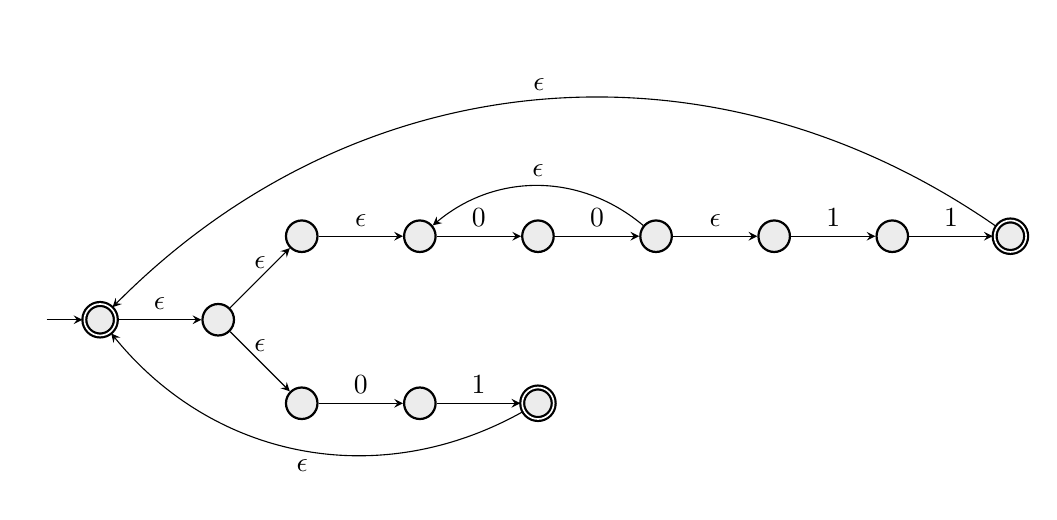
\begin{tikzpicture}[
                                styleSmall/.style={minimum size=4mm},
                                node distance=1.5cm,
                            ]
                            \node[state, initial, accepting, styleSmall] (q3e) {};
                            \node[state, styleSmall, right of=q3e] (qse) {};
                            \node[state, above right of=qse, styleSmall] (q0e) {};
                            \node[state, styleSmall, right of=q0e] (q0) {};
                            \node[state, right of=q0, styleSmall] (q01) {};
                            \node[state, right of=q01, styleSmall] (q02) {};
                            \node[state, right of=q02, styleSmall] (q1e) {};
                            \node[state, right of=q1e, styleSmall] (q11) {};
                            \node[state, accepting, right of=q11, styleSmall] (q12) {};
                            \node[state, below right of=qse, styleSmall] (qs1) {};
                            \node[state, right of=qs1, styleSmall] (qs2) {};
                            \node[state, accepting, right of=qs2, styleSmall] (qs3) {};
                            \draw
                            (q0e) edge[above] node{$\epsilon$} (q0)
                            (q0) edge[above] node{$0$} (q01)
                            (q01) edge[above] node{$0$} (q02)
                            (q02) edge[bend right=40, above] node{$\epsilon$} (q0)
                            (q02) edge[above] node{$\epsilon$} (q1e)
                            (q1e) edge[above] node{$1$} (q11)
                            (q11) edge[above] node{$1$} (q12)
                            (qse) edge[above] node{$\epsilon$} (q0e)
                            (qse) edge[above] node{$\epsilon$} (qs1)
                            (qs1) edge[above] node{$0$} (qs2)
                            (qs2) edge[above] node{$1$} (qs3)
                            (q3e) edge[above] node{$\epsilon$} (qse)
                            (q12) edge[bend right=40, above] node{$\epsilon$} (q3e)
                            (qs3) edge[bend left=40, below] node{$\epsilon$} (q3e);
                        \end{tikzpicture}
                        \caption{$(((00)^\ast(11)) \cup 01)^\ast$}
                    \end{figure}
              \item $\emptyset$
                    \begin{figure}[H]
                        \centering
                        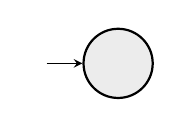
\begin{tikzpicture}
                            \node[state, initial] (q0) {};
                            \draw;
                        \end{tikzpicture}
                    \end{figure}
          \end{enumerate}

    \item [1.20]
          For each of the following languages, give two strings that are members and two strings that are not members—a total of four strings for each part. Assume the alphabet $\Sigma=\{a,b\}$ in all parts.
          \begin{enumerate}
              \item $a^\ast b^\ast $
                    \begin{table}[H]
                        \centering
                        \begin{tabular}{|c|c|}
                            \hline
                            Members    & Not Members \\
                            \hline
                            $\epsilon$ & $bbba$      \\
                            $ab$       & $abab$      \\
                            \hline
                        \end{tabular}
                    \end{table}
              \item $a(ba)^\ast b $
                    \begin{table}[H]
                        \centering
                        \begin{tabular}{|c|c|}
                            \hline
                            Members    & Not Members \\
                            \hline
                            $ab$       & $b$         \\
                            $aabababb$ & $aaab$      \\
                            \hline
                        \end{tabular}
                    \end{table}
              \item $a^\ast \cup b^\ast $
                    \begin{table}[H]
                        \centering
                        \begin{tabular}{|c|c|}
                            \hline
                            Members & Not Members \\
                            \hline
                            $aaa$   & $ab$        \\
                            $bbbb$  & $baba$      \\
                            \hline
                        \end{tabular}
                    \end{table}
              \item $(aaa)^\ast $
                    \begin{table}[H]
                        \centering
                        \begin{tabular}{|c|c|}
                            \hline
                            Members    & Not Members \\
                            \hline
                            $\epsilon$ & $b$         \\
                            $aaaaaa$   & $aa$        \\
                            \hline
                        \end{tabular}
                    \end{table}
              \item $\Sigma^\ast a\Sigma^\ast b\Sigma^\ast a\Sigma^\ast $
                    \begin{table}[H]
                        \centering
                        \begin{tabular}{|c|c|}
                            \hline
                            Members   & Not Members \\
                            \hline
                            $aba$     & $aaaa$      \\
                            $ababbbb$ & $bb$        \\
                            \hline
                        \end{tabular}
                    \end{table}
              \item $aba \cup bab $
                    \begin{table}[H]
                        \centering
                        \begin{tabular}{|c|c|}
                            \hline
                            Members & Not Members \\
                            \hline
                            $aba$   & $ababab$    \\
                            $bab$   & $abb$       \\
                            \hline
                        \end{tabular}
                    \end{table}
              \item $ (\epsilon  \cup a)b $
                    \begin{table}[H]
                        \centering
                        \begin{tabular}{|c|c|}
                            \hline
                            Members & Not Members \\
                            \hline
                            $b$     & $\epsilon$  \\
                            $ab$    & $aaba$      \\
                            \hline
                        \end{tabular}
                    \end{table}
              \item $(a\cup ba \cup bb)\Sigma$
                    \begin{table}[H]
                        \centering
                        \begin{tabular}{|c|c|}
                            \hline
                            Members & Not Members \\
                            \hline
                            $aa$    & $bbaa$      \\
                            $bbb$   & $abb$       \\
                            \hline
                        \end{tabular}
                    \end{table}
          \end{enumerate}

    \item [1.21]

          Use the procedure described in Lemma 1.60 to convert the following finite automata to regular expressions.
          \begin{enumerate}
              \item

                    \begin{figure}[H]
                        \centering
                        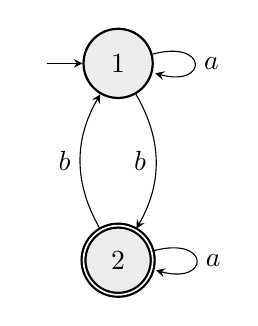
\begin{tikzpicture}
                            \node[state, initial] (q1) {1};
                            \node[state, below of=q1, accepting] (q2) {2};
                            \draw
                            (q1) edge[bend left, left] node{$b$} (q2)
                            (q2) edge[bend left, left] node{$b$} (q1)
                            (q1) edge[loop right] node{$a$} (q1)
                            (q2) edge[loop right] node{$a$} (q2)
                            ;
                        \end{tikzpicture}
                    \end{figure}

                    $b(a)^\ast b \cup a^\ast$
                    
              \item

                    \begin{figure}[H]
                        \centering
                        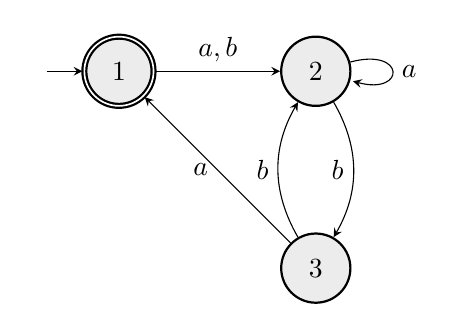
\begin{tikzpicture}
                            \node[state, initial, accepting] (q0) {1};
                            \node[state, right of=q0] (q1) {2};
                            \node[state, below of=q1] (q2) {3};;
                            \draw
                            (q1) edge[bend left, left] node{$b$} (q2)
                            (q2) edge[bend left, left] node{$b$} (q1)
                            (q2) edge[left, left] node{$a$} (q0)
                            (q0) edge[left, above] node{$a,b$} (q1)
                            (q1) edge[loop right] node{$a$} (q1)
                            ;
                        \end{tikzpicture}
                    \end{figure}

                    $a(a^\ast \cup bb)a \cup b(a^\ast \cup bb)a $
          \end{enumerate}
\end{enumerate}

\begin{enumerate}

    \item [1.22]
          In certain programming languages, comments appear between delimiters such as \slash\# and \#\slash .Let $C$ be the language of all valid delimited comment strings. A member of $C$ must begin with \slash \# and end with \# \slash but have no intervening \# \slash. For simplicity, assume that the alphabet for $C$ is $\Sigma=\{a,b,\text{/},\text{\#}\}$.
          \begin{enumerate}
              \item Give a DFA that recognizes $C$.
                    \begin{figure}[H]
                        \centering
                        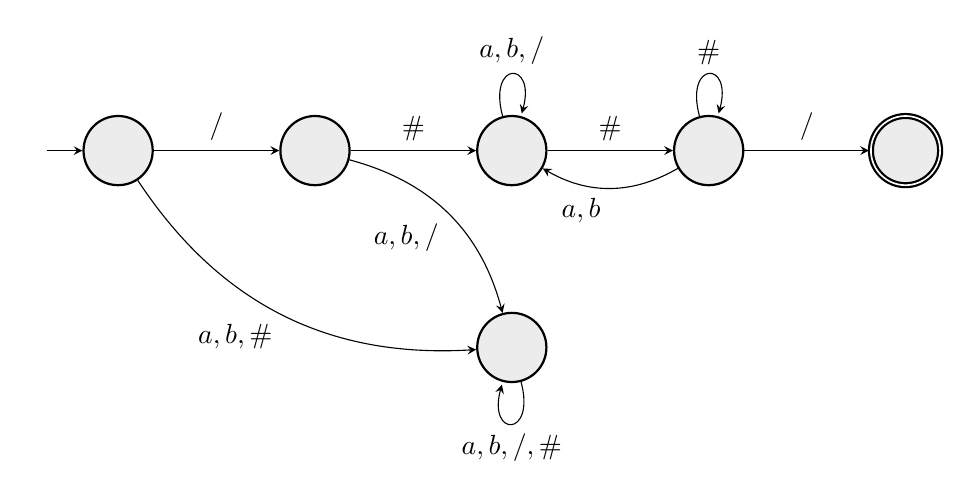
\begin{tikzpicture}[
                            ]
                            \node[state, initial] (q0) {};
                            \node[state, right of=q0] (q1) {};
                            \node[state, right of=q1] (q2) {};
                            \node[state, right of=q2] (q3) {};
                            \node[state, accepting, right of=q3] (q4) {};
                            \node[state, below of=q2] (q5) {};
                            \draw
                            (q0) edge[above] node{$\slash$} (q1)
                            (q1) edge[above] node{$\#$} (q2)
                            (q2) edge[loop above, above] node{$a,b,\slash$} (q2)
                            (q2) edge[above] node{$\#$} (q3)
                            (q3) edge[above] node{$\slash$} (q4)
                            (q0) edge[bend right, below left] node{$a,b,\#$} (q5)
                            (q1) edge[bend left, below left] node{$a,b,\slash$} (q5)
                            (q3) edge[bend left, below left] node{$a,b$} (q2)
                            (q3) edge[loop above, above] node{$\#$} (q3)
                            (q5) edge[loop below, below] node{$a,b,\slash,\#$} (q5);
                        \end{tikzpicture}
                        \caption{DFA recognizing $C$}
                    \end{figure}
              \item Give a regular expression that generates $C$.
                    $$\slash \#(a \cup b \cup \slash \cup (\#^\ast(a \cup b)))^\ast \# \slash $$
          \end{enumerate}
    \item [1.23]
          Let B be any language over the alphabet $\Sigma$. \\
          Prove that $B = B^+$ iff $BB \subseteq B$.

          Step 1\\
          Assume $B = B^+$. \\
          Let $x \in BB$. \\
          Then $x = uv$ for some $u,v \in B$. \\
          Since $B = B^+$, $u \in B^+$ and $v \in B^+$. \\
          Therefore $uv \in B^+$. \\
          Since $B^+ = B$, $uv \in B$. \\
          Therefore $BB \subseteq B$. \\
          \\
          Step 2\\
          Assume $BB \subseteq B$. \\
          Let $x \in B^+$. \\
          Then $x = uv$ for some $u,v \in B$. \\
          Since $BB \subseteq B$, $uv \in B$. \\
          Therefore $B^+ \subseteq B$. \\
          Since $B \subseteq B^+$ and $B^+ \subseteq B$ then $B = B^+$. \\
          Therefore $B = B^+$ iff $BB \subseteq B$. \\
    \item [1.24]
          A finite state transducer (FST) is a type of deterministic finite automaton whose output is a string and not just accept or reject. The following are state diagrams of finite state transducers $T_1$ and $T_2$.
          \begin{enumerate}
              \item $T_1$ on input $011$
                    \begin{table}[H]
                        \centering
                        \begin{tabular}{|c|c|}
                            \hline
                            States        & Output \\
                            \hline
                            $q1,q1,q1,q1$ & $000$  \\
                            \hline
                        \end{tabular}
                    \end{table}
              \item $T_1$ on input $211$
                    \begin{table}[H]
                        \centering
                        \begin{tabular}{|c|c|}
                            \hline
                            States        & Output \\
                            \hline
                            $q1,q2,q2,q2$ & $111$  \\
                            \hline
                        \end{tabular}
                    \end{table}
              \item $T_1$ on input $121$
                    \begin{table}[H]
                        \centering
                        \begin{tabular}{|c|c|}
                            \hline
                            States        & Output \\
                            \hline
                            $q1,q1,q2,q2$ & $011$  \\
                            \hline
                        \end{tabular}
                    \end{table}
              \item $T_1$ on input $0202$
                    \begin{table}[H]
                        \centering
                        \begin{tabular}{|c|c|}
                            \hline
                            States           & Output \\
                            \hline
                            $q1,q1,q2,q1,q2$ & $0101$ \\
                            \hline
                        \end{tabular}
                    \end{table}
              \item $T_2$ oninput $b$
                    \begin{table}[H]
                        \centering
                        \begin{tabular}{|c|c|}
                            \hline
                            States  & Output \\
                            \hline
                            $q1,q3$ & $1$    \\
                            \hline
                        \end{tabular}
                    \end{table}
              \item $T_2$ on input $bbab$
                    \begin{table}[H]
                        \centering
                        \begin{tabular}{|c|c|}
                            \hline
                            States           & Output \\
                            \hline
                            $q1,q3,q2,q3,q2$ & $1111$ \\
                            \hline
                        \end{tabular}
                    \end{table}
              \item $T_2$ on input $bbbbbb$
                    \begin{table}[H]
                        \centering
                        \begin{tabular}{|c|c|}
                            \hline
                            States                 & Output   \\
                            \hline
                            $q1,q3,q2,q1,q3,q2,q1$ & $110110$ \\
                            \hline
                        \end{tabular}
                    \end{table}
              \item $T_2$ on input $\epsilon$
                    \begin{table}[H]
                        \centering
                        \begin{tabular}{|c|c|}
                            \hline
                            States & Output     \\
                            \hline
                            $q1$   & $\epsilon$ \\
                            \hline
                        \end{tabular}
                    \end{table}
          \end{enumerate}
\end{enumerate}

\begin{enumerate}

    \item [1.31]
          For any string $w = w_1w_2\ldots w_n$, the reverse of $w$, written $w^R$, is the string $w$ in reverse order, $w_n \ldots w_2w_1$. For any language A, let $A^R = \{w^R ~|~ w \in A\}$. Show that if $A$ is regular, so is $A^R$.
          \\
          \\
          Let $$D = \{Q, \Sigma, \delta, q_0, F\}$$ be DFA recognizes $A$. We will construct a NFA $$D^R = \{Q^R, \Sigma, \delta^R, q^R_0, \{q_0\}\}$$ that recognizes $A^R$.

          $Q^R = Q \cup \{q^R_0\}$ where $q^R_0$ is new starting state connected with $\epsilon$-edges/transitions to each accepting state of $Q$ from $F$  \\
          $F^R = \{q_0\}$ (starting state from $D$ is accepting state of $D'$) \\
          $\delta^R(q, a) = \{p ~|~ \delta(p, a) = q\}$ \\
          and $\delta^R(q^R_0, \epsilon) = F$.





    \item [1.32]

          Let $\Sigma_3 = \Biggl \{\begin{bmatrix}0 \\ 0 \\ 0\end{bmatrix} , \begin{bmatrix}0 \\0 \\1 \end{bmatrix}, \begin{bmatrix}0 \\1 \\0\end{bmatrix} ,..., \begin{bmatrix}1 \\1 \\1\end{bmatrix} \Biggl \}$ . $\Sigma_3$ contains all size 3 columns of $0$'s and $1$'s. A string of symbols in $\Sigma_3$ gives three rows of $0$'s and $1$'s. Consider each row to be a binary number and let \\
          $B =\{w \in \Sigma^\ast_3 ~|~ \text{the bottom row of }~w~\text{is the sum of the top two rows}\}$. \\
          For example, $ \begin{bmatrix}0 \\0 \\1\end{bmatrix}  \begin{bmatrix}1 \\0 \\0\end{bmatrix} \begin{bmatrix} 1\\ 1\\ 0\end{bmatrix} \in B $, but $\begin{bmatrix}0 \\0 \\1\end{bmatrix} \begin{bmatrix}1\\ 0\\1\end{bmatrix} \notin B$. Show that $B$ is regular. (Hint: Working with $B^R$ is easier. You may assume the result claimed in Problem 1.31.)
          \\
          \\
          Let

          $ 0 = \begin{bmatrix}0 \\ 0 \\ 0\end{bmatrix} $
          $ 1 = \begin{bmatrix}0 \\ 0 \\ 1\end{bmatrix} $
          $ 2 = \begin{bmatrix}0 \\ 1 \\ 0\end{bmatrix} $
          $ \ldots $
          $ 7 = \begin{bmatrix}1 \\ 1 \\ 1\end{bmatrix} $
          be shorthand notation for each element of $\Sigma_3$.

          \begin{figure}[H]
              \centering
              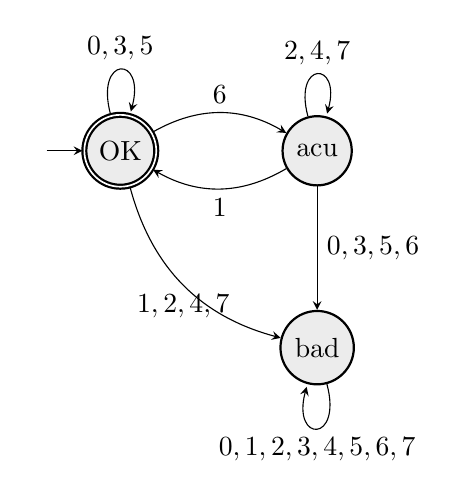
\begin{tikzpicture}[
                  ]
                  \node[state, accepting, initial] (q0) {OK};
                  \node[state, right of=q0] (qacc) {acu};
                  \node[state, below of=qacc] (qbad) {bad};
                  \draw
                  (q0) edge[bend left, above] node{$6$} (qacc)
                  (q0) edge[bend right, below] node{$1,2,4,7$} (qbad)
                  (qacc) edge[bend left, below] node{$1$} (q0)
                  (qacc) edge[right] node{$0,3,5,6$} (qbad)
                  (qacc) edge[loop above, above] node{$2,4,7$} (qacc)
                  (q0) edge[loop above, above] node{$0,3,5$} (q0)
                  (qbad) edge[loop below, below] node{$0,1,2,3,4,5,6,7$} (q0);
              \end{tikzpicture}
              \caption{DFA recognizing $\Sigma^{\ast R}_3 = B^R$}
          \end{figure}

          The DFA above recognizes $B^R$. By Problem 1.31, $B^R$ is regular. Since $B^R$ is regular, $B$ is regular as well.

    \item [1.33]
          Let $\Sigma_2 = \Biggl \{ \begin{bmatrix}0 \\0\end{bmatrix} , \begin{bmatrix}0 \\1\end{bmatrix} , \begin{bmatrix}1\\ 0\end{bmatrix}, \begin{bmatrix}1 \\1\end{bmatrix} \Biggl\}$. Here, $\Sigma_2$ contains all columns of $0$'s and $1$'s of height two. A string of symbols in $\Sigma_2$ gives two rows of $0$'s and $1$'s. Consider each row to be a binary number and let $C =\{w \in \Sigma^\ast_2~|~\text{the bottom row of }w \text{is three times the top row}\}$. For example, $\begin{bmatrix}0 \\0 \end{bmatrix}\begin{bmatrix}0\\ 1 \end{bmatrix}\begin{bmatrix}1 \\1 \end{bmatrix}\begin{bmatrix}0 \\0\end{bmatrix} \in C$, but $\begin{bmatrix}0 \\1\end{bmatrix} \begin{bmatrix}0\\ 1\end{bmatrix} \begin{bmatrix}1\\ 0\end{bmatrix} \notin C$. Show that $C$ is regular. (You may assume the result claimed in Problem 1.31.)

    \item [1.34]

          Let $\Sigma_2$ be the same as in Problem 1.33. Consider each row to be a binary number and let\\
          $D=\{ w \in \Sigma^\ast_2~ |~\text{the top row of }w~ \text{is a larger number than is the bottom row}\}$. For example, $\begin{bmatrix}0 \\0\end{bmatrix} \begin{bmatrix}1 \\0\end{bmatrix} \begin{bmatrix}1 \\1\end{bmatrix} \begin{bmatrix}0 \\0\end{bmatrix} \in D$, but $\begin{bmatrix}0\\ 0\end{bmatrix} \begin{bmatrix}0\\ 1\end{bmatrix} \begin{bmatrix} 1\\ 1\end{bmatrix} \begin{bmatrix} 0\\ 0\end{bmatrix} \notin D$. \\
          Show that $D$ is regular.
          \\ \\


\end{enumerate}

\begin{enumerate}

    \item [1.36]
          Let $B_n = \{a^k |  ~k~\text{is a multiple of} ~n\}$. Show that for each $n \ge 1$, the language $B_n$ is regular.

          Lets construct NFA accepting

          For $n = 2$:
          \begin{figure}[H]
              \centering
              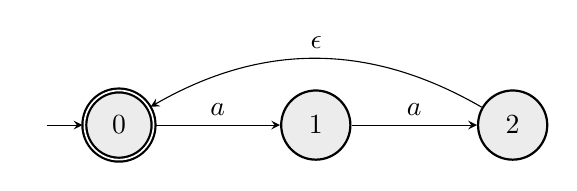
\begin{tikzpicture}[
                  ]
                  \node[state, initial, accepting] (q0) {$0$};
                  \node[state, right of=q0] (q1) {$1$};
                  \node[state, right of=q1] (q2) {$2$};
                  \draw
                  (q0) edge[above] node{$a$} (q1)
                  (q1) edge[above] node{$a$} (q2)
                  (q2) edge[bend right, above] node{$\epsilon$} (q0);
              \end{tikzpicture}
              \caption{NFA recognicing $B_2$}
          \end{figure}

          \begin{figure}[H]
              \centering
              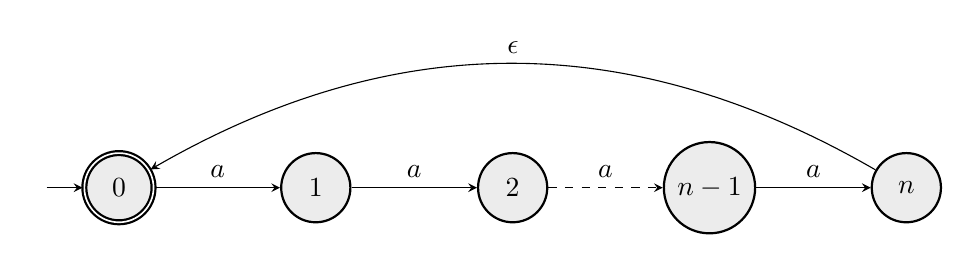
\begin{tikzpicture}[
                  ]
                  \node[state, initial, accepting] (q0) {$0$};
                  \node[state, right of=q0] (q1) {$1$};
                  \node[state, right of=q1] (q2) {$2$};
                  \node[state, right of=q2] (qe1) {$n-1$};
                  \node[state, right of=qe1] (qe) {$n$};
                  \draw
                  (q0) edge[above] node{$a$} (q1)
                  (q1) edge[above] node{$a$} (q2)
                  (q2) edge[above, dashed] node{$a$} (qe1)
                  (qe1) edge[above] node{$a$} (qe)
                  (qe) edge[bend right, above] node{$\epsilon$} (q0);
              \end{tikzpicture}
              \caption{NFA recognicing $B_n$}
          \end{figure}

    \item [1.37]
          Let $C_n = \{x~ |~ x~ \text{is a binary number that is a multiple of} ~n\}$. Show that for each $n \ge 1$, the language $C_n$ is regular.

          Lets build $DFA_C$ recognizing $C_n$:

          $DFA_C = (Q, \Sigma, \delta, q_0, F)$
          \begin{itemize}
              \item $Q = \{0', 1', 2', \ldots, (n-1)'\}$
              \item $\Sigma = \{0, 1\}$
              \item $q_0 = 0'$
              \item $F = \{0'\}$
              \item $\delta$ is defined as follows:
                    \begin{align*}
                        \delta(q', 0) & = 2q \Mod{n}                                   \\
                        \delta(q', 1) & = (2q + 1) \Mod{n} = (2q \Mod{n} + 1 ) \Mod{n}
                    \end{align*}
                    where q is the integer part of $q'$.
          \end{itemize}
          We build DFA recognizing $C_n$ so $C_n$ is regular.

          Idea

          $i\text{-th}$ state represents integers which modulo from dividing by $n$ is $i$, because $n$ is multiple of $n$.

          \begin{figure}[H]
              \centering
              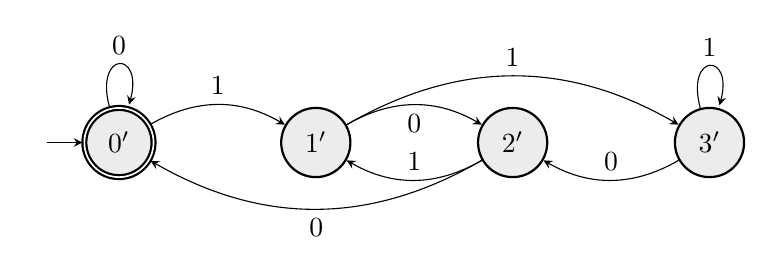
\begin{tikzpicture}[
                  ]
                  \node[state, initial, accepting] (q0) {$0'$};
                  \node[state, right of=q0] (q1) {$1'$};
                  \node[state, right of=q1] (q2) {$2'$};
                  \node[state, right of=q2] (q3) {$3'$};
                  \draw
                  (q0) edge[loop above] node{$0$} (q0)
                  (q0) edge[bend left, above] node{$1$} (q1)
                  (q1) edge[bend left, below] node{$0$} (q2)
                  (q1) edge[bend left, above] node{$1$} (q3)
                  (q2) edge[bend left, below] node{$0$} (q0)
                  (q2) edge[bend left, above] node{$1$} (q1)
                  (q3) edge[bend left, above] node{$0$} (q2)
                  (q3) edge[loop above] node{$1$} (q3);
              \end{tikzpicture}
              \caption{$DFA_C$ for $n = 4$}
          \end{figure}

          \begin{table}[H]
              \centering
              \begin{tabular}{|r|r|r|r|}
                  \hline
                  $0'$: mod 4 = 0 & $1'$: mod  4 = 1 & $2'$: mod 4 = 2 & $3'$: mod 4 = 3 \\
                  \hline
                  $0 = (0)_2$     & $1 = (1)_2$      & $2 = (10)_2$    & $3 = (11)_2$    \\
                  $4 = (100)_2$   & $5 = (101)_2$    & $6 = (110)_2$   & $7 = (111)_2$   \\
                  $8 = (1000)_2$  & $9 = (1001)_2$   & $10 = (1010)_2$ & $11 = (1011)_2$ \\
                  \ldots          & \ldots           & \ldots          & \ldots          \\
                  \hline
              \end{tabular}
          \end{table}

    \item [1.38]

          An all-NFA $M$ is a 5-tuple $(Q,\Sigma,\delta,q_0,F)$ that accepts $x \in \Sigma^\ast$ if every possible state that $M$ could be in after reading input $x$ is a state from $F$. Note, in contrast, that an ordinary NFA accepts a string if some state among these possible states is an accept state. Prove that all-NFAs recognize the class of regular languages.

          In procedure to change NFA to DFA just change step which marks state as accepting when state of DFA corresponds to states of NFA with at least one is acccepting to accepting only when all states are accepting.

          Now we have DFA accepting the same language as all-NFA $M$ so language is regular.
    \item [1.39]
          The construction in Theorem 1.54 shows that every GNFA is equivalent to a GNFA with only two states. We can show that an opposite phenomenon occurs for DFAs. Prove that for every $k > 1$, a language $A_k \subseteq \{0,1\}^\ast$ exists that is recognized by a DFA with $k$ states but not by one with only $k-1$ states.
    \item [1.40]
          Recall that string $x$ is a \textbf{prefix} of string $y$ if a string $z$ exists where $xz = y$, and that $x$ is a \textbf{proper prefix} of $y$ if in addition $x \neq y$. In each of the following parts, we define an operation on a language $A$. Show that the class of regular languages is closed under that operation.
          \begin{itemize}
              \item $L = \text{NOPREFIX}(A)=\{w \in A~|~\text{no proper prefix of } w~ \text{is a member of}~ A\}$.

                    Let be DFA $M = (Q, \Sigma, \delta, q_0, F)$ recognizes A (as A is regular language).

                    We need to construct $L$ which contains strings so that DFA $M$ will go to accepting state only at the end of processing string. In other words for all $w = w_1w_2\ldots w_n \in A$, $\delta(q_{i-1}, w_i) = q_{i}$ and $q_i \in F$ only for $i = n$.

                    DFA $M_{NOPREFIX} = (Q \cup {q_f}, \Sigma, \delta_{NOPREFIX}, q_0, F)$

                    where $\delta_{NOPREFIX}(q, a) = \delta(q, a)$ for $q \in Q$ and $\delta_{NOPREFIX}(q, a) = q_f$ for $q \in F$.
                    

              \item $\text{NOEXTEND}(A)=\{w \in A~|~w~ \text{is not the proper prefix of any string in}~ A\}$.

                During processing string $w$ DFA $M$ can't go from accepting state to another accepting state by any possible way.

                DFA $M_{NOEXTEND} = (Q, \Sigma, \delta, q_0, F_{NOEXTEND})$

                where $F_{NOEXTEND} = F - F'$

                where $F'$ is set of states which can be reached from accepting state by any possible way.

                To build $F'$ lets go from all accepting states and mark all states which can be reached from them. Then $F'$ is set of all marked states. We can stop after $\overline{Q}$ steps where $\overline{Q}$ is number of states in DFA $M$. Each step we go every $a \in \Sigma$ from every accepting state or state reached from previous step.
          \end{itemize}
\end{enumerate}

\begin{enumerate}

      \item [1.41]
            
            For languages $A$ and $B$,let the \textbf{perfect shuffle} of $A$ and $B$ be the language $\{w~|~ w = a_1b_1\ldots a_kb_k , \text{where} a_1\ldots a_k \in A \text{and} b_1 \ldots b_k \in B, each a_i,b_i \in \Sigma\}$. Show that the class of regular languages is closed under perfect shuffle.
            
            TODO - double check this solution
            
            Let $A$ and $B$ be regular languages. Then there exist DFAs $M_A$ and $M_B$ that accept $A$ and $B$, respectively. We construct a DFA $M$ that accepts the perfect shuffle of $A$ and $B$.
            
            Let $M_A = (Q_A,\Sigma,\delta_A,q_{0A},F_A)$ and $M_B = (Q_B,\Sigma,\delta_B,q_{0B},F_B)$. Let $Q = Q_A \times Q_B$, $q_0 = (q_{0A},q_{0B})$, and $F = F_A \times F_B$. The transition function $\delta$ is defined as follows: for each $q \in Q$ and $a \in \Sigma$, $\delta(q,a) = (\delta_A(q_A,a),\delta_B(q_B,a))$.
            
            We claim that $L(M) = A \circ B$. Let $w = a_1b_1\ldots a_kb_k \in A \circ B$. Then there exists a sequence of states $r_0,r_1,\ldots,r_k$ such that $r_0 = q_0$, $r_k \in F$, and $\delta(r_{i-1},a_i) = r_i$ for $i = 1,\ldots,k$. Let $r_i = (r_{iA},r_{iB})$. Then $r_{iA} \in Q_A$ and $r_{iB} \in Q_B$. Since $r_k \in F$, $r_{kA} \in F_A$ and $r_{kB} \in F_B$. Thus $a_1\ldots a_k \in A$ and $b_1\ldots b_k \in B$. Therefore $w \in A \circ B$.
            
            Conversely, let $w = a_1\ldots a_kb_1\ldots b_k \in A \circ B$. Then $a_1\ldots a_k \in A$ and $b_1\ldots b_k \in B$. Let $r_i = (r_{iA},r_{iB})$ for $i = 0,\ldots,k$. Then $r_0 = q_0$, $r_k \in F$, and $\delta(r_{i-1},a_i) = r_i$ for $i = 1,\ldots,k$. Therefore $w \in L(M)$.
            
            
      \item [1.42]
            
            For languages $A$ and $B$, let the \textbf{shuffle} of $A$ and $B$ be the language $\{w~|~ w = a_1b_1\ldots a_kb_k, where a_1 \ldots a_k \in A \text{and} b_1 \ldots b_k \in B\text{, each }a_i,b_i \in \Sigma^\ast\}$. Show that the class of regular languages is closed under \textbf{shuffle}.
            
      \item [1.43]
            
            Let $A$ be any language. Define $\text{DROP-OUT}(A)$ to be the language containing all strings that can be obtained by removing one symbol from a string in $A$. Thus,
            
            $\text{DROP-OUT}(A)=\{xz ~|~ xyz \in A~ \text{where}~ x,z \in \Sigma^\ast,y \in \Sigma\}$.
            
            Show that the class of regular languages is closed under the $\text{DROP-OUT}$ operation. Give both a proof by picture and a more formal proof by construction as in Theorem 1.47.
            
      \item [1.44]
      \item [1.45]
      \item [1.46]
      \item [1.47]
      \item [1.48]
      \item [1.49]
            
            \begin{itemize}
                  \item Let $B =\{1^ky~|~ y \in \{0,1\}^\ast \text{and} ~y~ \text{contains at least}~ k~ 1\text{s, for}~ k \ge 1\}$. Show that $B$ is a regular language.
                  \item Let $C =\{1^ky~|~y \in\{0,1\}^\ast \text{and}~ y ~\text{contains at most} ~k~ 1\text{s, for}~ k \ge 1\}$. Show that $C$ isn’t a regular language.
            \end{itemize}
            
\end{enumerate}

\begin{enumerate}

      \item [1.50]
            
            Read the informal definition of the finite state transducer given in Exercise 1.24. Prove that no FST can output $w^R$ for every input $w$ if the input and output alphabets are $\{0,1\}$.
            
      \item [1.51]
            
            Let $x$ and $y$ be strings and let $L$ be any language. We say that $x$ and $y$ are \textbf{distinguishable by $L$} if some string $z$ exists whereby exactly one of the strings $xz$ and $yz$ is a member of $L$; otherwise, for every string $z$, we have $xz \in L$ whenever $yz \in L$ and we say that $x$ and $y$ are \textbf{indistinguishable by $L$}. 
            
            If $x$ and $y$ are indistinguishable by $L$, we write $x \equiv_{L} y$ . Show that $\equiv_{L}$ is an equivalence relation.
            
      \item [1.52]
            
            \textbf{Myhill–Nerode theorem}. 
            
            Refer to Problem 1.51. Let $L$ be a language and let $X$ be a set of strings. Say that $X$ is \textbf{pairwise distinguishable by L} if every two distinct strings in $X$ are distinguishable by L. Define the index of $L$ to be the maximum number of elements in any set that is pairwise distinguishable by $L$. The index of $L$ may befinite or infinite. 
            
            \begin{enumerate}
                  \item Show that if $L$ is recognized by a $DFA$ with $k$ states, $L$ has index at most $k$.
                  \item Show that if the index of $L$ is a finite number $k$, it is recognized by a $DFA$ with $k$ states.
                  \item Conclude that $L$ is regular iff it has finite index. Moreover, its index is the size of the smallest $DFA$ recognizing it.
            \end{enumerate}
            
      \item [1.53]
            
            Let $\Sigma = \{0,1,+,=\}$ and 
            
            $$ADD = \{x=y+z~|~x,y,z~\text{are binary integers, and}~ x~ \text{is the sum of}~ y ~\text{and}~ z\}.$$
            
            Show that $ADD$ is not regular.
            
      \item [1.54]
            
            Consider the language $F = \{a^i b^j c^k ~|~ i,j,k \geq 0~ \text{and if}~ i=1~ \text{then}~~ j = k\}$. 
            \begin{enumerate}
                  \item Show that $F$ is not regular.
                  \item Show that $F$ acts like a regular language in the pumping lemma. In other words, give a pumping length $p$ and demonstrate that $F$ satisfies the three conditions of the pumping lemma for this value of $p$.
                  \item Explain why parts (a) and (b) do not contradict the pumping lemma.
                        
            \end{enumerate}
            
      \item [1.55]
            
            The pumping lemma says that every regular language has a pumping length $p$, such that every string in the language can be pumped if it has length $p$ or more. If $p$ is a pumping length for language $A$, so is any length $p' \ge p$.The minimum pumping length for $A$ is the smallest $p$ that is a pumping length for $A$. For example, if $A=01^\ast$,the minimum pumping length is 2. The reason is that the string $s = 0$ is in $A$ and has length $1$ yet $s$ cannot be pumped; but any string in $A$ of length $2$ or more contains a $1$ and hence can be pumped by dividing it so that $x = 0, y = 1$, and $z$ is the rest. For each of the following languages, give the minimum pumping length and justify your answer.
            
            \begin{enumerate}
                  \item $0001^\ast$
                        
                        Shortest word in language is $000$ but it cannot be pumped. So, minimum pumping length is 4 as $0001$ can be pumped.
                        
                  \item $0^\ast 1^\ast$
                        
                        Minimum pumping length is 1 as $0$ or $1$ can be pumped. Any longer word can be pumped by pumping $0$'s or $1$'s. 
                        
                  \item $001 \cup 0^\ast 1^\ast$
                        
                        Minimum pumping length is 1 as $0$ or $1$ can be pumped. Any longer word can be pumped by pumping $0$'s or $1$'s. Even word $001$ can be pumped by pumping $0$'s or $1$'s as it belongs also to second of two languages sums to that language.
                        
                  \item $0^\ast 1^+ 0^+ 1^+ 1^\ast \cup 10^\ast1$
                        
                        Minimum pumping length has to be greater than 2 as $11$ cannot be pumped. 
                        Minimum pumping length is 3 as words of form $10^{+}1$ can be pumped. Also words from first part of union (with minimum length of 3) can be pumped by pumping $0$'s or $1$'s (as $101$ belong also to second part of union but cannot be pumped within only first part of union).
                        
                  \item $(01)^\ast$
                        
                        Minimum pumping length is 2 as $01$ can be pumped.
                        
                  \item $\epsilon$
                        
                        Minimum pumping length is 1 as $\epsilon$ with length 0 cannot be pumped.
                        
                  \item $1^\ast01^\ast01^\ast$
                        
                        Minimum pumping length is greater than 2 as $00$ can be pumped. Minimum pumping length is 3 as every word with at least one $1$ can be pumped.
                        
                  \item $10(11^\ast0)^\ast0$
                        
                        Minimum pumping length has to be greater than 3 as $100$ cannot be pumped. Minimum pumping length is 4 as words of form $10110$ can be pumped (which is of length 5 but 4 also satisfies pumping lemma requirements).
                        
                  \item $1011$
                        
                        Minimum pumping length is 5 as $1011$ (with length = 4) cannot be pumped.
                        
                  \item $\Sigma^\ast$
                        
                        Minimum pumping length is 1 as any word can be pumped. Assuming empty string $\epsilon$ cannot be pumped as stated in selected solutions (but not sure from which lemma assumptions it can be stated).
                        
            \end{enumerate}
            
      \item [1.56]
            
            If $A$ is a set of natural numbers and $k$ is a natural number greater than $1$, let $B_k(A)=\{w~|~w~ \text{is the representation in base}~k~\text{of some number in} A\}$. Here, we do not allow leading $0$s in the representation of a number. For example, $B_2({3,5})=\{11,101\}$ and $B_3({3,5})=\{10,12\}$. Give an example of a set $A$ for which $B_2(A)$ is regular but $B_3(A)$ is not regular. 
            
            Prove that your example works.
            
      \item [1.57]
            
            If $A$ is any language, let $A_{\frac{1}{2}-}$ be the set of all first halves of strings in A so that $A_{\frac{1}{2}-} = \{x~|~ \text{for some}~ y, |x| = |y| ~\text{and}~ xy \in A\}$. 
            
            Show that if $A$ is regular, then so is $A_{\frac{1}{2}-}$.
            
      \item [1.58]
            
            If $A$ is any language, let $A_{\frac{1}{3}-\frac{1}{3}}$ be the set of all strings in A with their middle thirds removed so that $A_{\frac{1}{3}-\frac{1}{3}} = \{xz~|~ \text{for some}~ y, |x| = |y| = |z|~ \text{and}~ xyz \in A\}$. Show that if $A$ is regular, then $A_{\frac{1}{3}-\frac{1}{3}}$ is not necessarily regular.
            
      \item [1.59]
            
            Let $M = (Q,\Sigma, \delta, q_0, F)$ be a DFA and let $h$ be a state of $M$ called its “home”. A synchronizing sequence for $M$ and $h$ is a string $s \in \Sigma^\ast$ where $\delta(q,s)=h$ for every $q \in Q$. 
            
            (Here we have extended $\delta$ to strings, so that $\delta(q,s)$ equals the state where $M$ ends up when $M$ starts at state $q$ and reads input $s$.) 
            
            Say that $M$ is synchronizable if it has a synchronizing sequence for some state $h$. Prove that if $M$ is a $k$-state synchronizable DFA, then it has a synchronizing sequence of length at most $k^3$. 
            
            Can you improve upon this bound?
            
\end{enumerate}



\end{document}
